\documentclass[12pt]{article}
\usepackage[spanish]{babel}
\usepackage[utf8]{inputenc}
\usepackage{amsmath}
\usepackage{graphicx}
\usepackage{booktabs}
\usepackage{array}
\usepackage{multirow}
\usepackage{float}
\usepackage{longtable}
\usepackage{subcaption}
\usepackage{wrapfig}
\usepackage{tikz}
\usetikzlibrary{arrows.meta, positioning, shapes.geometric}
\title{Proyecto 3: Reemplazo de Equipos}
\author{Emily Sanchez \\ Viviana Vargas \\[1cm] Curso: Investigación de Operaciones \\ II Semestre 2025}
\date{\today}

\begin{document}

\maketitle
\newpage
\section*{Problema de Reemplazo de Equipos}
El algoritmo de reemplazo de equipos se utiliza en Investigación de Operaciones para decidir cuándo conviene reemplazar una máquina o equipo que se deteriora con el tiempo.\\
La idea básica es comparar dos tipos de costos:\\
\begin{itemize}
\item \textbf{Costo de mantener el equipo actual:} Incluye reparaciones, mantenimiento y costos de operación, que normalmente aumentan con los años de uso.\\
\item \textbf{Costo de reemplazarlo por uno nuevo:} Incluye el costo inicial de adquisición y el valor de rescate (lo obtenido al vender el equipo viejo).\\
\end{itemize}
El objetivo es minimizar el costo promedio anual (o el valor presente de los costos) a lo largo del tiempo.\\
\textbf{Variaciones comunes del problema:}\\
\begin{itemize}
\item \textbf{Ganancias por año:} La productividad del equipo disminuye con la edad, afectando los ingresos.\\
\item \textbf{Inflación:} Los precios de adquisición y mantenimiento cambian según el año.\\
\item \textbf{Nuevas tecnologías:} Equipos más modernos pueden ofrecer mejores rendimientos y menores costos operativos.\\
\end{itemize}
\textbf{Fórmula del costo:} $C_{t,j} = \text{Compra} + \sum \text{Mantenimiento}_k - \sum \text{Profit}_k - \text{Venta}_{j-t}$\\
\textbf{Algoritmo:} Programación Dinámica \\
\textbf{Función recursiva:} $g(t) = \min\limits_{j=t+1}^{\min(t+\text{vida útil}, n)} \{C_{t,j} + g(j)\}$ con $g(n) = 0$\\

\section*{Datos del Problema}
\begin{itemize}
\item Costo inicial (compra): \$1000.00
\item Plazo del proyecto: 3 años
\item Vida útil del equipo: 5 años
\end{itemize}

\begin{table}[H]
\centering
\caption{Datos del equipo por año de uso}
\begin{tabular}{cccc}
\toprule
Año de Uso & Mantenimiento & Valor Residual & Beneficio \\
\midrule
1 & \$60.00 & \$975.00 & \$100.00 \\
2 & \$70.00 & \$860.00 & \$90.00 \\
3 & \$80.00 & \$750.00 & \$80.00 \\
\bottomrule
\end{tabular}
\end{table}

\clearpage
\section*{Cálculo de Costos $C_{t,j}$}
\begin{longtable}{cccc}
\caption{Cálculo detallado de costos por período} \\
\toprule
Período (t-j) & Duración & Fórmula & Costo \\
\midrule
\endfirsthead
\multicolumn{4}{c}{\tablename\ \thetable\ -- Continúa} \\
\toprule
Período (t-j) & Duración & Fórmula & Costo \\
\midrule
\endhead
\midrule
\multicolumn{4}{r}{Continúa en la siguiente página} \\
\endfoot
\bottomrule
\endlastfoot
0-1 & 1 año & $1000 + 60 - 100 - 975$ & \$-15.00 \\
0-2 & 2 años & $1000 + 60 + 70 - 100 - 90 - 860$ & \$80.00 \\
0-3 & 3 años & $1000 + 60 + 70 + 80 - 100 - 90 - 80 - 750$ & \$190.00 \\
1-2 & 1 año & $1000 + 60 - 100 - 975$ & \$-15.00 \\
1-3 & 2 años & $1000 + 60 + 70 - 100 - 90 - 860$ & \$80.00 \\
2-3 & 1 año & $1000 + 60 - 100 - 975$ & \$-15.00 \\
\end{longtable}

\clearpage
\section*{Cálculo de $g(t)$ (Programación Dinámica)}
\begin{itemize}
\item $g(3) = 0$ (caso base)
\item $g(2) = \min\{ \mathbf{C_{2,3} + g(3) = -15.00}\} = \$-15.00$ \textbf{(j=3)}
\item $g(1) = \min\{ \mathbf{C_{1,2} + g(2) = -30.00}, C_{1,3} + g(3) = 80.00\} = \$-30.00$ \textbf{(j=2)}
\item $g(0) = \min\{ \mathbf{C_{0,1} + g(1) = -45.00}, C_{0,2} + g(2) = 65.00, C_{0,3} + g(3) = 190.00\} = \$-45.00$ \textbf{(j=1)}
\end{itemize}

\subsection*{Empates}
Se han resaltado en \textbf{negrita} las opciones óptimas.\\
\textbf{No se encontraron empates.} Existe una única estrategia óptima para cada año de inicio.\\
\clearpage
\section*{Solución Óptima}
\textbf{Costo mínimo total:} \$-45.00\\
\textbf{Planes óptimos encontrados:} 1
\subsection*{Grafos de Planes Óptimos}
A continuación se presentan los grafos de \emph{saltos de rana} para cada plan óptimo encontrado.

\begin{figure}[H]
\centering
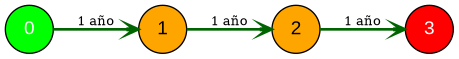
\includegraphics[width=0.8\textwidth]{Reemplazo5x2_plan_1.png}
\caption{Plan Óptimo 1: \texttt{0-1-2-3}}
\label{fig:plan1}
\end{figure}

\textbf{Plan 1:} \texttt{0-1-2-3}
\begin{itemize}\small
\item Período 0-1: 1 año, Costo: \$-15.00
\item Período 1-2: 1 año, Costo: \$-15.00
\item Período 2-3: 1 año, Costo: \$-15.00
\end{itemize}

\end{document}
